
% Default to the notebook output style

    


% Inherit from the specified cell style.




    
\documentclass[11pt]{article}

    
    
    \usepackage[T1]{fontenc}
    % Nicer default font (+ math font) than Computer Modern for most use cases
    \usepackage{mathpazo}

    % Basic figure setup, for now with no caption control since it's done
    % automatically by Pandoc (which extracts ![](path) syntax from Markdown).
    \usepackage{graphicx}
    % We will generate all images so they have a width \maxwidth. This means
    % that they will get their normal width if they fit onto the page, but
    % are scaled down if they would overflow the margins.
    \makeatletter
    \def\maxwidth{\ifdim\Gin@nat@width>\linewidth\linewidth
    \else\Gin@nat@width\fi}
    \makeatother
    \let\Oldincludegraphics\includegraphics
    % Set max figure width to be 80% of text width, for now hardcoded.
    \renewcommand{\includegraphics}[1]{\Oldincludegraphics[width=.8\maxwidth]{#1}}
    % Ensure that by default, figures have no caption (until we provide a
    % proper Figure object with a Caption API and a way to capture that
    % in the conversion process - todo).
    \usepackage{caption}
    \DeclareCaptionLabelFormat{nolabel}{}
    \captionsetup{labelformat=nolabel}

    \usepackage{adjustbox} % Used to constrain images to a maximum size 
    \usepackage{xcolor} % Allow colors to be defined
    \usepackage{enumerate} % Needed for markdown enumerations to work
    \usepackage{geometry} % Used to adjust the document margins
    \usepackage{amsmath} % Equations
    \usepackage{amssymb} % Equations
    \usepackage{textcomp} % defines textquotesingle
    % Hack from http://tex.stackexchange.com/a/47451/13684:
    \AtBeginDocument{%
        \def\PYZsq{\textquotesingle}% Upright quotes in Pygmentized code
    }
    \usepackage{upquote} % Upright quotes for verbatim code
    \usepackage{eurosym} % defines \euro
    \usepackage[mathletters]{ucs} % Extended unicode (utf-8) support
    \usepackage[utf8x]{inputenc} % Allow utf-8 characters in the tex document
    \usepackage{fancyvrb} % verbatim replacement that allows latex
    \usepackage{grffile} % extends the file name processing of package graphics 
                         % to support a larger range 
    % The hyperref package gives us a pdf with properly built
    % internal navigation ('pdf bookmarks' for the table of contents,
    % internal cross-reference links, web links for URLs, etc.)
    \usepackage{hyperref}
    \usepackage{longtable} % longtable support required by pandoc >1.10
    \usepackage{booktabs}  % table support for pandoc > 1.12.2
    \usepackage[inline]{enumitem} % IRkernel/repr support (it uses the enumerate* environment)
    \usepackage[normalem]{ulem} % ulem is needed to support strikethroughs (\sout)
                                % normalem makes italics be italics, not underlines
    

    
    
    % Colors for the hyperref package
    \definecolor{urlcolor}{rgb}{0,.145,.698}
    \definecolor{linkcolor}{rgb}{.71,0.21,0.01}
    \definecolor{citecolor}{rgb}{.12,.54,.11}

    % ANSI colors
    \definecolor{ansi-black}{HTML}{3E424D}
    \definecolor{ansi-black-intense}{HTML}{282C36}
    \definecolor{ansi-red}{HTML}{E75C58}
    \definecolor{ansi-red-intense}{HTML}{B22B31}
    \definecolor{ansi-green}{HTML}{00A250}
    \definecolor{ansi-green-intense}{HTML}{007427}
    \definecolor{ansi-yellow}{HTML}{DDB62B}
    \definecolor{ansi-yellow-intense}{HTML}{B27D12}
    \definecolor{ansi-blue}{HTML}{208FFB}
    \definecolor{ansi-blue-intense}{HTML}{0065CA}
    \definecolor{ansi-magenta}{HTML}{D160C4}
    \definecolor{ansi-magenta-intense}{HTML}{A03196}
    \definecolor{ansi-cyan}{HTML}{60C6C8}
    \definecolor{ansi-cyan-intense}{HTML}{258F8F}
    \definecolor{ansi-white}{HTML}{C5C1B4}
    \definecolor{ansi-white-intense}{HTML}{A1A6B2}

    % commands and environments needed by pandoc snippets
    % extracted from the output of `pandoc -s`
    \providecommand{\tightlist}{%
      \setlength{\itemsep}{0pt}\setlength{\parskip}{0pt}}
    \DefineVerbatimEnvironment{Highlighting}{Verbatim}{commandchars=\\\{\}}
    % Add ',fontsize=\small' for more characters per line
    \newenvironment{Shaded}{}{}
    \newcommand{\KeywordTok}[1]{\textcolor[rgb]{0.00,0.44,0.13}{\textbf{{#1}}}}
    \newcommand{\DataTypeTok}[1]{\textcolor[rgb]{0.56,0.13,0.00}{{#1}}}
    \newcommand{\DecValTok}[1]{\textcolor[rgb]{0.25,0.63,0.44}{{#1}}}
    \newcommand{\BaseNTok}[1]{\textcolor[rgb]{0.25,0.63,0.44}{{#1}}}
    \newcommand{\FloatTok}[1]{\textcolor[rgb]{0.25,0.63,0.44}{{#1}}}
    \newcommand{\CharTok}[1]{\textcolor[rgb]{0.25,0.44,0.63}{{#1}}}
    \newcommand{\StringTok}[1]{\textcolor[rgb]{0.25,0.44,0.63}{{#1}}}
    \newcommand{\CommentTok}[1]{\textcolor[rgb]{0.38,0.63,0.69}{\textit{{#1}}}}
    \newcommand{\OtherTok}[1]{\textcolor[rgb]{0.00,0.44,0.13}{{#1}}}
    \newcommand{\AlertTok}[1]{\textcolor[rgb]{1.00,0.00,0.00}{\textbf{{#1}}}}
    \newcommand{\FunctionTok}[1]{\textcolor[rgb]{0.02,0.16,0.49}{{#1}}}
    \newcommand{\RegionMarkerTok}[1]{{#1}}
    \newcommand{\ErrorTok}[1]{\textcolor[rgb]{1.00,0.00,0.00}{\textbf{{#1}}}}
    \newcommand{\NormalTok}[1]{{#1}}
    
    % Additional commands for more recent versions of Pandoc
    \newcommand{\ConstantTok}[1]{\textcolor[rgb]{0.53,0.00,0.00}{{#1}}}
    \newcommand{\SpecialCharTok}[1]{\textcolor[rgb]{0.25,0.44,0.63}{{#1}}}
    \newcommand{\VerbatimStringTok}[1]{\textcolor[rgb]{0.25,0.44,0.63}{{#1}}}
    \newcommand{\SpecialStringTok}[1]{\textcolor[rgb]{0.73,0.40,0.53}{{#1}}}
    \newcommand{\ImportTok}[1]{{#1}}
    \newcommand{\DocumentationTok}[1]{\textcolor[rgb]{0.73,0.13,0.13}{\textit{{#1}}}}
    \newcommand{\AnnotationTok}[1]{\textcolor[rgb]{0.38,0.63,0.69}{\textbf{\textit{{#1}}}}}
    \newcommand{\CommentVarTok}[1]{\textcolor[rgb]{0.38,0.63,0.69}{\textbf{\textit{{#1}}}}}
    \newcommand{\VariableTok}[1]{\textcolor[rgb]{0.10,0.09,0.49}{{#1}}}
    \newcommand{\ControlFlowTok}[1]{\textcolor[rgb]{0.00,0.44,0.13}{\textbf{{#1}}}}
    \newcommand{\OperatorTok}[1]{\textcolor[rgb]{0.40,0.40,0.40}{{#1}}}
    \newcommand{\BuiltInTok}[1]{{#1}}
    \newcommand{\ExtensionTok}[1]{{#1}}
    \newcommand{\PreprocessorTok}[1]{\textcolor[rgb]{0.74,0.48,0.00}{{#1}}}
    \newcommand{\AttributeTok}[1]{\textcolor[rgb]{0.49,0.56,0.16}{{#1}}}
    \newcommand{\InformationTok}[1]{\textcolor[rgb]{0.38,0.63,0.69}{\textbf{\textit{{#1}}}}}
    \newcommand{\WarningTok}[1]{\textcolor[rgb]{0.38,0.63,0.69}{\textbf{\textit{{#1}}}}}
    
    
    % Define a nice break command that doesn't care if a line doesn't already
    % exist.
    \def\br{\hspace*{\fill} \\* }
    % Math Jax compatability definitions
    \def\gt{>}
    \def\lt{<}
    % Document parameters
    \title{????????v1}
    
    
    

    % Pygments definitions
    
\makeatletter
\def\PY@reset{\let\PY@it=\relax \let\PY@bf=\relax%
    \let\PY@ul=\relax \let\PY@tc=\relax%
    \let\PY@bc=\relax \let\PY@ff=\relax}
\def\PY@tok#1{\csname PY@tok@#1\endcsname}
\def\PY@toks#1+{\ifx\relax#1\empty\else%
    \PY@tok{#1}\expandafter\PY@toks\fi}
\def\PY@do#1{\PY@bc{\PY@tc{\PY@ul{%
    \PY@it{\PY@bf{\PY@ff{#1}}}}}}}
\def\PY#1#2{\PY@reset\PY@toks#1+\relax+\PY@do{#2}}

\expandafter\def\csname PY@tok@w\endcsname{\def\PY@tc##1{\textcolor[rgb]{0.73,0.73,0.73}{##1}}}
\expandafter\def\csname PY@tok@c\endcsname{\let\PY@it=\textit\def\PY@tc##1{\textcolor[rgb]{0.25,0.50,0.50}{##1}}}
\expandafter\def\csname PY@tok@cp\endcsname{\def\PY@tc##1{\textcolor[rgb]{0.74,0.48,0.00}{##1}}}
\expandafter\def\csname PY@tok@k\endcsname{\let\PY@bf=\textbf\def\PY@tc##1{\textcolor[rgb]{0.00,0.50,0.00}{##1}}}
\expandafter\def\csname PY@tok@kp\endcsname{\def\PY@tc##1{\textcolor[rgb]{0.00,0.50,0.00}{##1}}}
\expandafter\def\csname PY@tok@kt\endcsname{\def\PY@tc##1{\textcolor[rgb]{0.69,0.00,0.25}{##1}}}
\expandafter\def\csname PY@tok@o\endcsname{\def\PY@tc##1{\textcolor[rgb]{0.40,0.40,0.40}{##1}}}
\expandafter\def\csname PY@tok@ow\endcsname{\let\PY@bf=\textbf\def\PY@tc##1{\textcolor[rgb]{0.67,0.13,1.00}{##1}}}
\expandafter\def\csname PY@tok@nb\endcsname{\def\PY@tc##1{\textcolor[rgb]{0.00,0.50,0.00}{##1}}}
\expandafter\def\csname PY@tok@nf\endcsname{\def\PY@tc##1{\textcolor[rgb]{0.00,0.00,1.00}{##1}}}
\expandafter\def\csname PY@tok@nc\endcsname{\let\PY@bf=\textbf\def\PY@tc##1{\textcolor[rgb]{0.00,0.00,1.00}{##1}}}
\expandafter\def\csname PY@tok@nn\endcsname{\let\PY@bf=\textbf\def\PY@tc##1{\textcolor[rgb]{0.00,0.00,1.00}{##1}}}
\expandafter\def\csname PY@tok@ne\endcsname{\let\PY@bf=\textbf\def\PY@tc##1{\textcolor[rgb]{0.82,0.25,0.23}{##1}}}
\expandafter\def\csname PY@tok@nv\endcsname{\def\PY@tc##1{\textcolor[rgb]{0.10,0.09,0.49}{##1}}}
\expandafter\def\csname PY@tok@no\endcsname{\def\PY@tc##1{\textcolor[rgb]{0.53,0.00,0.00}{##1}}}
\expandafter\def\csname PY@tok@nl\endcsname{\def\PY@tc##1{\textcolor[rgb]{0.63,0.63,0.00}{##1}}}
\expandafter\def\csname PY@tok@ni\endcsname{\let\PY@bf=\textbf\def\PY@tc##1{\textcolor[rgb]{0.60,0.60,0.60}{##1}}}
\expandafter\def\csname PY@tok@na\endcsname{\def\PY@tc##1{\textcolor[rgb]{0.49,0.56,0.16}{##1}}}
\expandafter\def\csname PY@tok@nt\endcsname{\let\PY@bf=\textbf\def\PY@tc##1{\textcolor[rgb]{0.00,0.50,0.00}{##1}}}
\expandafter\def\csname PY@tok@nd\endcsname{\def\PY@tc##1{\textcolor[rgb]{0.67,0.13,1.00}{##1}}}
\expandafter\def\csname PY@tok@s\endcsname{\def\PY@tc##1{\textcolor[rgb]{0.73,0.13,0.13}{##1}}}
\expandafter\def\csname PY@tok@sd\endcsname{\let\PY@it=\textit\def\PY@tc##1{\textcolor[rgb]{0.73,0.13,0.13}{##1}}}
\expandafter\def\csname PY@tok@si\endcsname{\let\PY@bf=\textbf\def\PY@tc##1{\textcolor[rgb]{0.73,0.40,0.53}{##1}}}
\expandafter\def\csname PY@tok@se\endcsname{\let\PY@bf=\textbf\def\PY@tc##1{\textcolor[rgb]{0.73,0.40,0.13}{##1}}}
\expandafter\def\csname PY@tok@sr\endcsname{\def\PY@tc##1{\textcolor[rgb]{0.73,0.40,0.53}{##1}}}
\expandafter\def\csname PY@tok@ss\endcsname{\def\PY@tc##1{\textcolor[rgb]{0.10,0.09,0.49}{##1}}}
\expandafter\def\csname PY@tok@sx\endcsname{\def\PY@tc##1{\textcolor[rgb]{0.00,0.50,0.00}{##1}}}
\expandafter\def\csname PY@tok@m\endcsname{\def\PY@tc##1{\textcolor[rgb]{0.40,0.40,0.40}{##1}}}
\expandafter\def\csname PY@tok@gh\endcsname{\let\PY@bf=\textbf\def\PY@tc##1{\textcolor[rgb]{0.00,0.00,0.50}{##1}}}
\expandafter\def\csname PY@tok@gu\endcsname{\let\PY@bf=\textbf\def\PY@tc##1{\textcolor[rgb]{0.50,0.00,0.50}{##1}}}
\expandafter\def\csname PY@tok@gd\endcsname{\def\PY@tc##1{\textcolor[rgb]{0.63,0.00,0.00}{##1}}}
\expandafter\def\csname PY@tok@gi\endcsname{\def\PY@tc##1{\textcolor[rgb]{0.00,0.63,0.00}{##1}}}
\expandafter\def\csname PY@tok@gr\endcsname{\def\PY@tc##1{\textcolor[rgb]{1.00,0.00,0.00}{##1}}}
\expandafter\def\csname PY@tok@ge\endcsname{\let\PY@it=\textit}
\expandafter\def\csname PY@tok@gs\endcsname{\let\PY@bf=\textbf}
\expandafter\def\csname PY@tok@gp\endcsname{\let\PY@bf=\textbf\def\PY@tc##1{\textcolor[rgb]{0.00,0.00,0.50}{##1}}}
\expandafter\def\csname PY@tok@go\endcsname{\def\PY@tc##1{\textcolor[rgb]{0.53,0.53,0.53}{##1}}}
\expandafter\def\csname PY@tok@gt\endcsname{\def\PY@tc##1{\textcolor[rgb]{0.00,0.27,0.87}{##1}}}
\expandafter\def\csname PY@tok@err\endcsname{\def\PY@bc##1{\setlength{\fboxsep}{0pt}\fcolorbox[rgb]{1.00,0.00,0.00}{1,1,1}{\strut ##1}}}
\expandafter\def\csname PY@tok@kc\endcsname{\let\PY@bf=\textbf\def\PY@tc##1{\textcolor[rgb]{0.00,0.50,0.00}{##1}}}
\expandafter\def\csname PY@tok@kd\endcsname{\let\PY@bf=\textbf\def\PY@tc##1{\textcolor[rgb]{0.00,0.50,0.00}{##1}}}
\expandafter\def\csname PY@tok@kn\endcsname{\let\PY@bf=\textbf\def\PY@tc##1{\textcolor[rgb]{0.00,0.50,0.00}{##1}}}
\expandafter\def\csname PY@tok@kr\endcsname{\let\PY@bf=\textbf\def\PY@tc##1{\textcolor[rgb]{0.00,0.50,0.00}{##1}}}
\expandafter\def\csname PY@tok@bp\endcsname{\def\PY@tc##1{\textcolor[rgb]{0.00,0.50,0.00}{##1}}}
\expandafter\def\csname PY@tok@fm\endcsname{\def\PY@tc##1{\textcolor[rgb]{0.00,0.00,1.00}{##1}}}
\expandafter\def\csname PY@tok@vc\endcsname{\def\PY@tc##1{\textcolor[rgb]{0.10,0.09,0.49}{##1}}}
\expandafter\def\csname PY@tok@vg\endcsname{\def\PY@tc##1{\textcolor[rgb]{0.10,0.09,0.49}{##1}}}
\expandafter\def\csname PY@tok@vi\endcsname{\def\PY@tc##1{\textcolor[rgb]{0.10,0.09,0.49}{##1}}}
\expandafter\def\csname PY@tok@vm\endcsname{\def\PY@tc##1{\textcolor[rgb]{0.10,0.09,0.49}{##1}}}
\expandafter\def\csname PY@tok@sa\endcsname{\def\PY@tc##1{\textcolor[rgb]{0.73,0.13,0.13}{##1}}}
\expandafter\def\csname PY@tok@sb\endcsname{\def\PY@tc##1{\textcolor[rgb]{0.73,0.13,0.13}{##1}}}
\expandafter\def\csname PY@tok@sc\endcsname{\def\PY@tc##1{\textcolor[rgb]{0.73,0.13,0.13}{##1}}}
\expandafter\def\csname PY@tok@dl\endcsname{\def\PY@tc##1{\textcolor[rgb]{0.73,0.13,0.13}{##1}}}
\expandafter\def\csname PY@tok@s2\endcsname{\def\PY@tc##1{\textcolor[rgb]{0.73,0.13,0.13}{##1}}}
\expandafter\def\csname PY@tok@sh\endcsname{\def\PY@tc##1{\textcolor[rgb]{0.73,0.13,0.13}{##1}}}
\expandafter\def\csname PY@tok@s1\endcsname{\def\PY@tc##1{\textcolor[rgb]{0.73,0.13,0.13}{##1}}}
\expandafter\def\csname PY@tok@mb\endcsname{\def\PY@tc##1{\textcolor[rgb]{0.40,0.40,0.40}{##1}}}
\expandafter\def\csname PY@tok@mf\endcsname{\def\PY@tc##1{\textcolor[rgb]{0.40,0.40,0.40}{##1}}}
\expandafter\def\csname PY@tok@mh\endcsname{\def\PY@tc##1{\textcolor[rgb]{0.40,0.40,0.40}{##1}}}
\expandafter\def\csname PY@tok@mi\endcsname{\def\PY@tc##1{\textcolor[rgb]{0.40,0.40,0.40}{##1}}}
\expandafter\def\csname PY@tok@il\endcsname{\def\PY@tc##1{\textcolor[rgb]{0.40,0.40,0.40}{##1}}}
\expandafter\def\csname PY@tok@mo\endcsname{\def\PY@tc##1{\textcolor[rgb]{0.40,0.40,0.40}{##1}}}
\expandafter\def\csname PY@tok@ch\endcsname{\let\PY@it=\textit\def\PY@tc##1{\textcolor[rgb]{0.25,0.50,0.50}{##1}}}
\expandafter\def\csname PY@tok@cm\endcsname{\let\PY@it=\textit\def\PY@tc##1{\textcolor[rgb]{0.25,0.50,0.50}{##1}}}
\expandafter\def\csname PY@tok@cpf\endcsname{\let\PY@it=\textit\def\PY@tc##1{\textcolor[rgb]{0.25,0.50,0.50}{##1}}}
\expandafter\def\csname PY@tok@c1\endcsname{\let\PY@it=\textit\def\PY@tc##1{\textcolor[rgb]{0.25,0.50,0.50}{##1}}}
\expandafter\def\csname PY@tok@cs\endcsname{\let\PY@it=\textit\def\PY@tc##1{\textcolor[rgb]{0.25,0.50,0.50}{##1}}}

\def\PYZbs{\char`\\}
\def\PYZus{\char`\_}
\def\PYZob{\char`\{}
\def\PYZcb{\char`\}}
\def\PYZca{\char`\^}
\def\PYZam{\char`\&}
\def\PYZlt{\char`\<}
\def\PYZgt{\char`\>}
\def\PYZsh{\char`\#}
\def\PYZpc{\char`\%}
\def\PYZdl{\char`\$}
\def\PYZhy{\char`\-}
\def\PYZsq{\char`\'}
\def\PYZdq{\char`\"}
\def\PYZti{\char`\~}
% for compatibility with earlier versions
\def\PYZat{@}
\def\PYZlb{[}
\def\PYZrb{]}
\makeatother


    % Exact colors from NB
    \definecolor{incolor}{rgb}{0.0, 0.0, 0.5}
    \definecolor{outcolor}{rgb}{0.545, 0.0, 0.0}



    
    % Prevent overflowing lines due to hard-to-break entities
    \sloppy 
    % Setup hyperref package
    \hypersetup{
      breaklinks=true,  % so long urls are correctly broken across lines
      colorlinks=true,
      urlcolor=urlcolor,
      linkcolor=linkcolor,
      citecolor=citecolor,
      }
    % Slightly bigger margins than the latex defaults
    
    \geometry{verbose,tmargin=1in,bmargin=1in,lmargin=1in,rmargin=1in}
    
    

    \begin{document}
    
    
    \maketitle
    
    

    
    \hypertarget{ux8baeux9898}{%
\section{议题}\label{ux8baeux9898}}

\begin{itemize}
\item
  ``人工智能''能做什么?
\item
  怎么学习``人工智能''?
\item
  他是如何工作的?
\item
  几个简单的范例
\end{itemize}

    人工智能? 机器学习? 深度学习? 
\includegraphics{img/twitter.png}

    机器学习是实现人工智能的一种方法,而深度学习是机器学习中的一种技术;
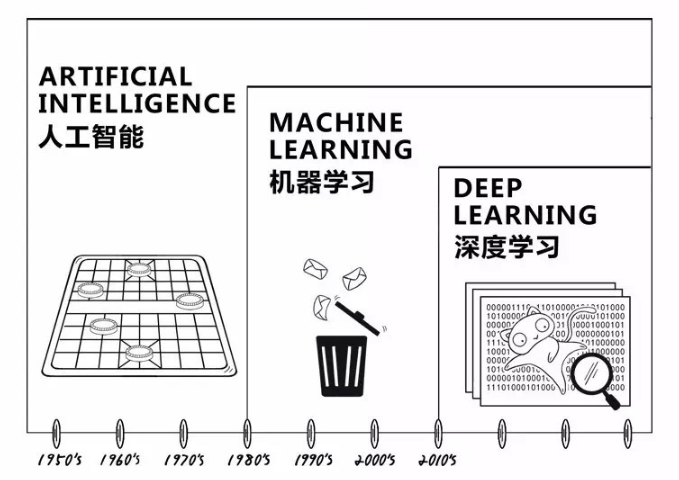
\includegraphics{img/aimldl.png}

    \hypertarget{ux76d1ux7763ux5b66ux4e60}{%
\subsection{监督学习}\label{ux76d1ux7763ux5b66ux4e60}}


\includegraphics{img/supervised.png}

从\textbf{有标记}的训练数据中推导出预测函数。有标记的训练数据是指每个训练实例都包括输入和期望的输出。简单的说,用我们\textbf{已经知道答案}的数据进行学习与训练;

    在机器学习领域中,我们通常把输入称为\texttt{数据},答案称为\texttt{标签}
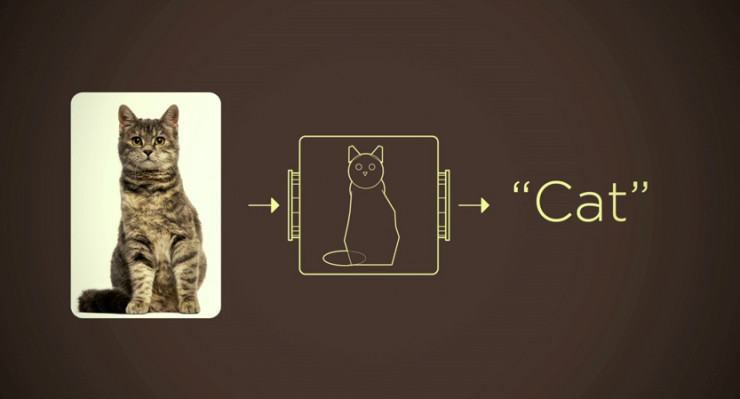
\includegraphics{img/label.jpg}

    对于监督学习,拥有多样化高质量的数据是最大的挑战

\includegraphics{img/cat.jpg}

    ImageNet有超过150万标注图像数据约2万多个分类
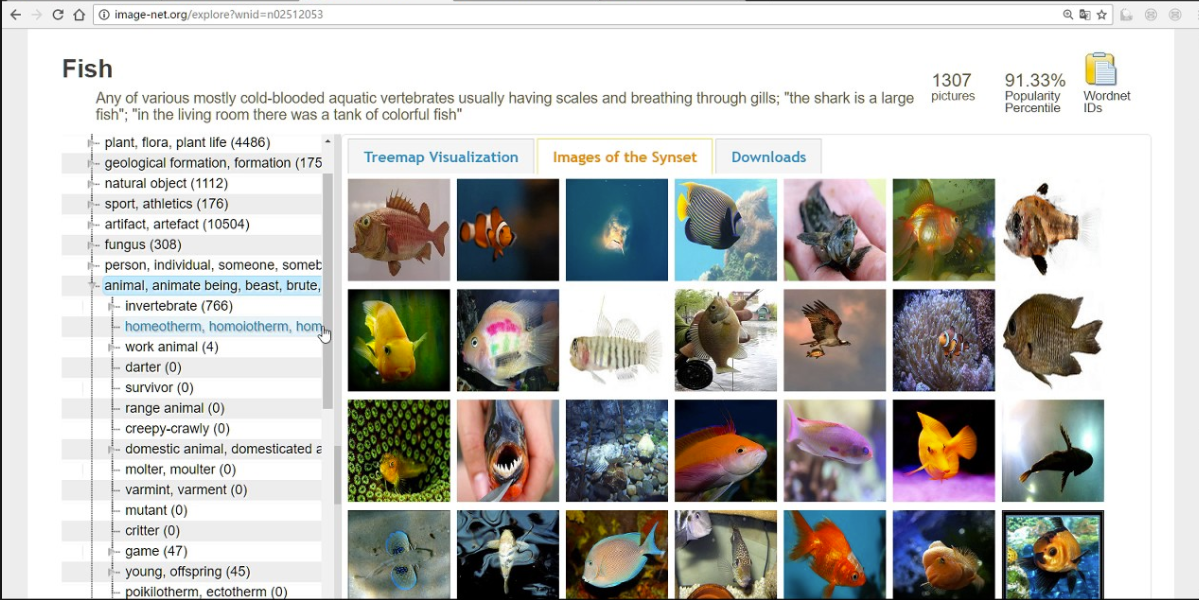
\includegraphics{img/imagenet.png}

    \begin{Verbatim}[commandchars=\\\{\}]
{\color{incolor}In [{\color{incolor}1}]:} \PY{o}{\PYZpc{}\PYZpc{}HTML}
        \PY{p}{\PYZlt{}}\PY{n+nt}{video} \PY{n+na}{width}\PY{o}{=}\PY{l+s}{\PYZdq{}600\PYZdq{}} \PY{n+na}{height}\PY{o}{=}\PY{l+s}{\PYZdq{}400\PYZdq{}} \PY{n+na}{controls}\PY{p}{\PYZgt{}} \PY{p}{\PYZlt{}}\PY{n+nt}{source} \PY{n+na}{src}\PY{o}{=}\PY{l+s}{\PYZdq{}img/YOLOv3.mp4\PYZdq{}} \PY{n+na}{type}\PY{o}{=}\PY{l+s}{\PYZdq{}video/mp4\PYZdq{}}\PY{p}{\PYZgt{}}\PY{p}{\PYZlt{}}\PY{p}{/}\PY{n+nt}{video}\PY{p}{\PYZgt{}}
\end{Verbatim}


    
    \begin{verbatim}
<IPython.core.display.HTML object>
    \end{verbatim}

    
    \hypertarget{ux65e0ux76d1ux7763ux5b66ux4e60}{%
\subsection{无监督学习}\label{ux65e0ux76d1ux7763ux5b66ux4e60}}

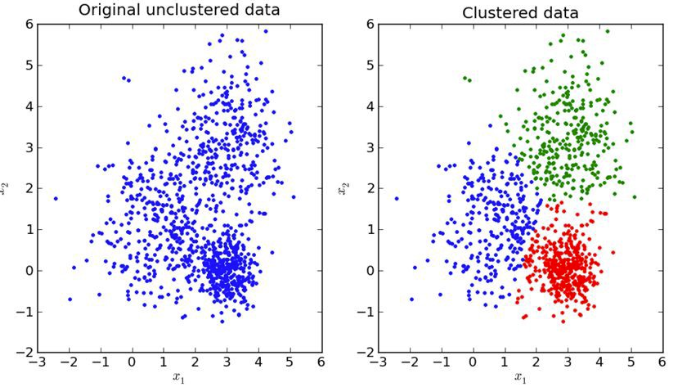
\includegraphics{img/unsupervised.png}
从\textbf{无标记}的训练数据中推断结论。用于发现隐藏的模式或者对数据进行分组。简单的说:给定数据,寻找隐藏的结构

    \hypertarget{word-embeddingux8bcdux5d4cux5165ux5411ux91cf}{%
\subsubsection{Word
Embedding(词嵌入向量)}\label{word-embeddingux8bcdux5d4cux5165ux5411ux91cf}}

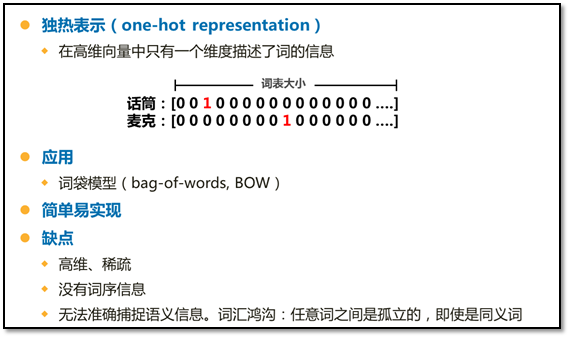
\includegraphics{img/one-hot.png}

    wiki:

猫,通常指家猫,在现代汉语中也昵称猫咪、咪咪、喵星人\ldots{}\ldots{}.现在,\texttt{猫}成为世界上最为广泛的\textbf{宠物}之一

犬,现代俗称为狗,一种常见的犬科哺乳动物\ldots{}\ldots{}\ldots{}\ldots{}.\texttt{狗}可用作陪伴、警用、军用、做\textbf{宠物}

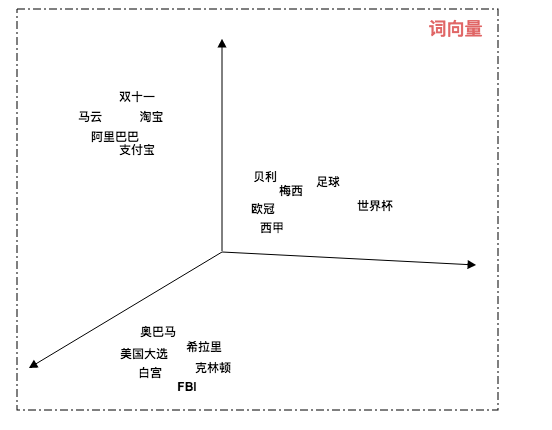
\includegraphics{img/wordspace.png}

    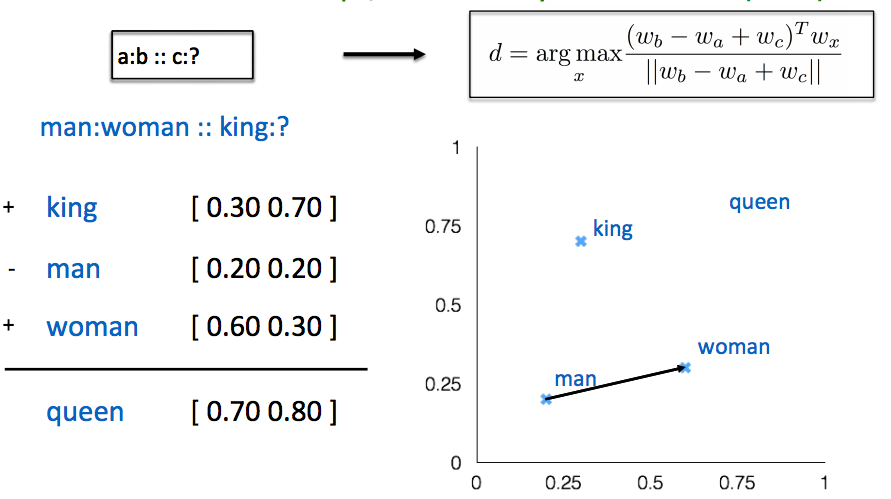
\includegraphics{img/wordcal.png}

    \hypertarget{ux4e07ux7269ux7686ux53efembedding}{%
\subsubsection{万物皆可embedding}\label{ux4e07ux7269ux7686ux53efembedding}}

基于电商浏览记录、抖音视频观看记录、搜索记录构建上下文,并进行向量嵌入计算
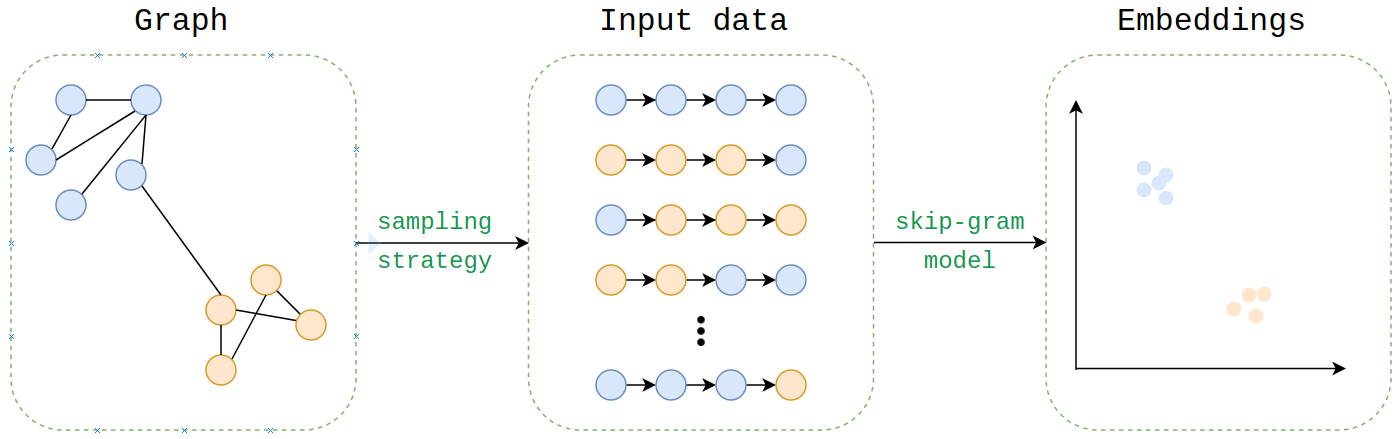
\includegraphics{img/commodityembedding.png}

    \hypertarget{ux5bf9ux6297ux751fux6210ux7f51ux7edcgan}{%
\subsection{对抗生成网络(GAN)}\label{ux5bf9ux6297ux751fux6210ux7f51ux7edcgan}}

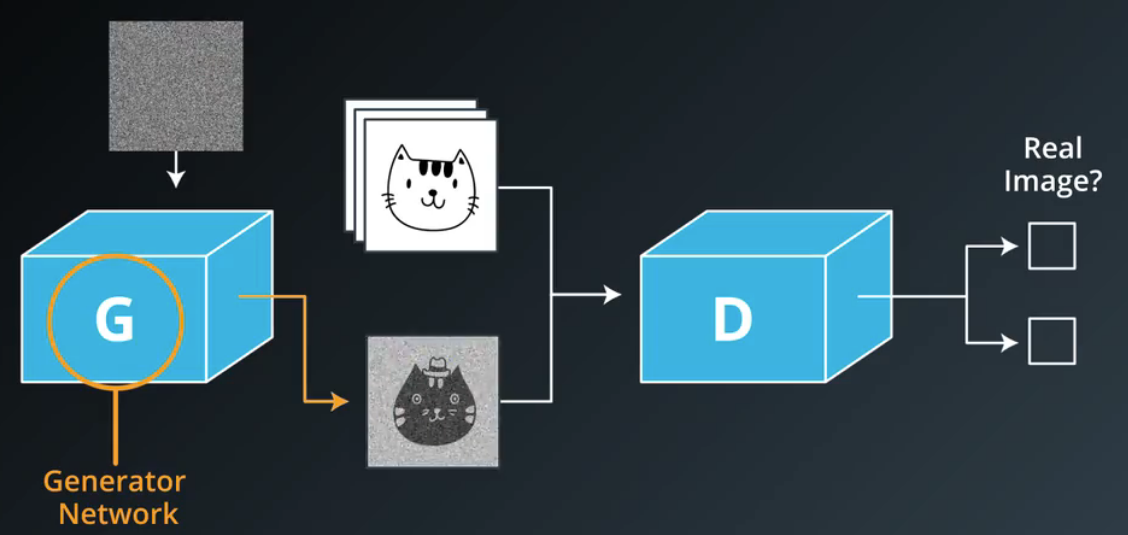
\includegraphics{img/GAN.png}

    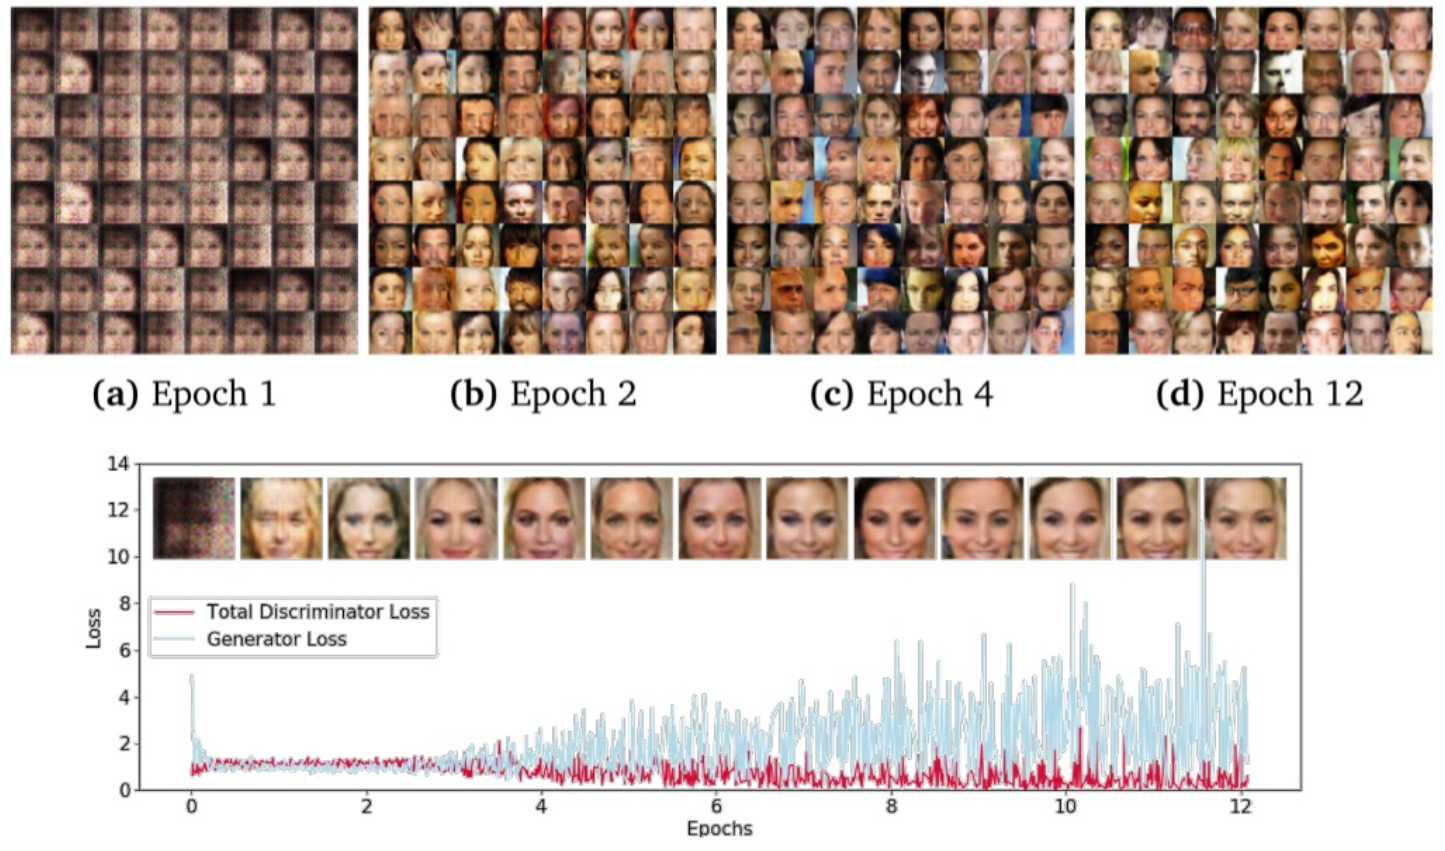
\includegraphics{img/celeA.png}

    你能辨别出下图中哪些是真人哪些是GAN生成的照片吗?
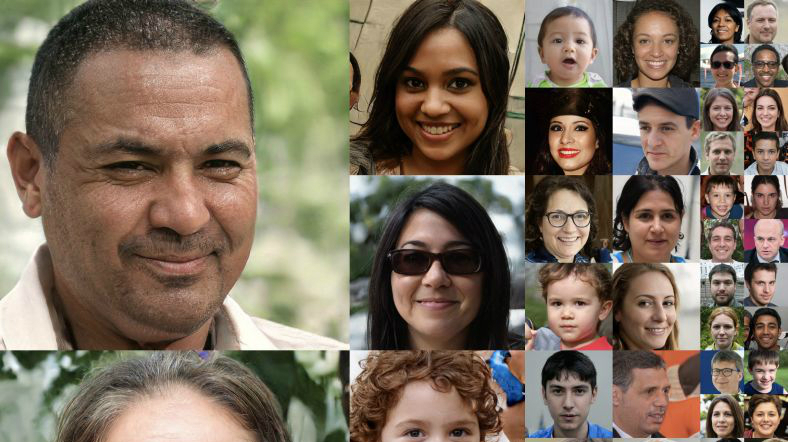
\includegraphics{img/ganface.jpg}

    \hypertarget{ux5f3aux5316ux5b66ux4e60}{%
\subsection{强化学习}\label{ux5f3aux5316ux5b66ux4e60}}

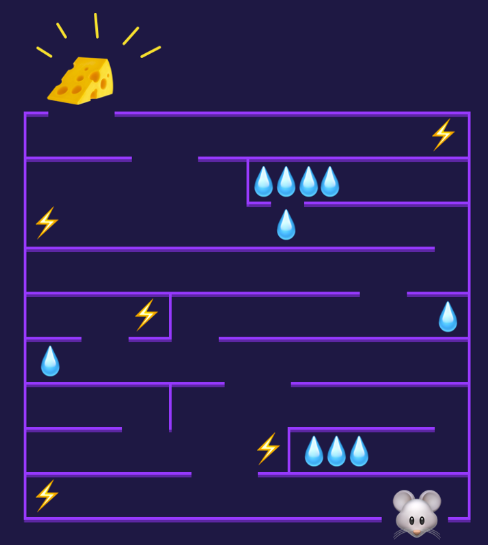
\includegraphics{img/rl.png}

强化学习,强调让程序学习如何基于环境而行动,以取得最大化的预期利益。

    电脑通过自我博弈学会了 补刀、勾兵、卡兵等操作

    \begin{Verbatim}[commandchars=\\\{\}]
{\color{incolor}In [{\color{incolor}4}]:} \PY{o}{\PYZpc{}\PYZpc{}HTML}
        \PY{p}{\PYZlt{}}\PY{n+nt}{video} \PY{n+na}{width}\PY{o}{=}\PY{l+s}{\PYZdq{}600\PYZdq{}} \PY{n+na}{height}\PY{o}{=}\PY{l+s}{\PYZdq{}400\PYZdq{}} \PY{n+na}{controls}\PY{p}{\PYZgt{}} \PY{p}{\PYZlt{}}\PY{n+nt}{source} \PY{n+na}{src}\PY{o}{=}\PY{l+s}{\PYZdq{}img/dota2.mp4\PYZdq{}} \PY{n+na}{type}\PY{o}{=}\PY{l+s}{\PYZdq{}video/mp4\PYZdq{}}\PY{p}{\PYZgt{}}\PY{p}{\PYZlt{}}\PY{p}{/}\PY{n+nt}{video}\PY{p}{\PYZgt{}}
\end{Verbatim}


    
    \begin{verbatim}
<IPython.core.display.HTML object>
    \end{verbatim}

    
    \hypertarget{ux673aux5668ux5b66ux4e60ux7684ux8fb9ux754c}{%
\section{机器学习的边界}\label{ux673aux5668ux5b66ux4e60ux7684ux8fb9ux754c}}

机器学习目前三大方向

\begin{itemize}
\tightlist
\item
  计算机视觉
\item
  语音识别
\item
  自然语言处理
\end{itemize}

    谷歌语音助理

语音(输入)--\textgreater{} 文字 --\textgreater{} 对话模型
--\textgreater{} 文字 --\textgreater{} 语音(输出)

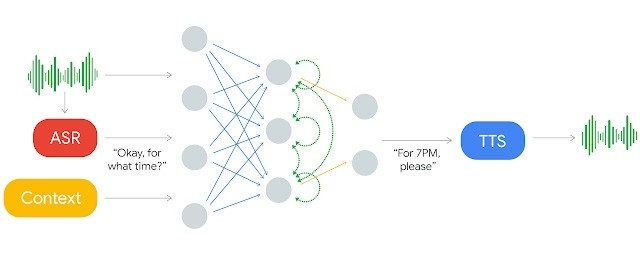
\includegraphics{img/duplex.jpg}

    ``推荐餐厅,不要日本菜!'' 结果推荐的都是日本菜

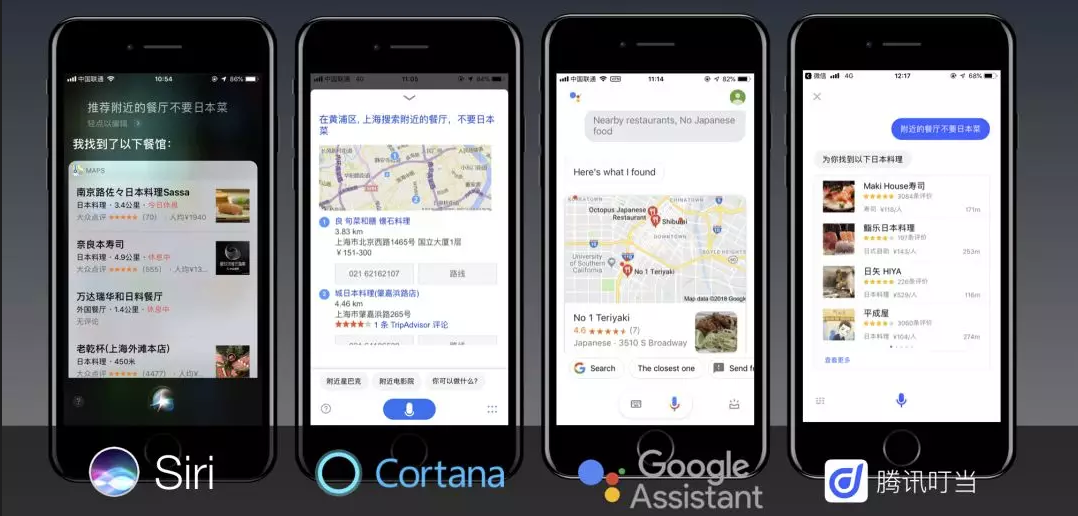
\includegraphics{img/ai_test.png}

    \href{https://mp.weixin.qq.com/s/tFcVohNjdhvBE_INQk9muQ}{人工智障:你看到的AI与智能无关}

今天还是1月6日,但2年前的今天,你与交往了5年的女友分手了,之后一直对她念念不忘,也没有交往新人。

你和往日一样,进电梯的,刚要关门的时候,匆忙进来的一个人,要关的门又打开了。就是你2年前分手的那位前女友。她进门时看到只有你们两,她抬头看了一下你,然后又低头找楼层电梯了:

\begin{quote}
这时她说:``你好''。

你也回答: ``你好''。
\end{quote}

    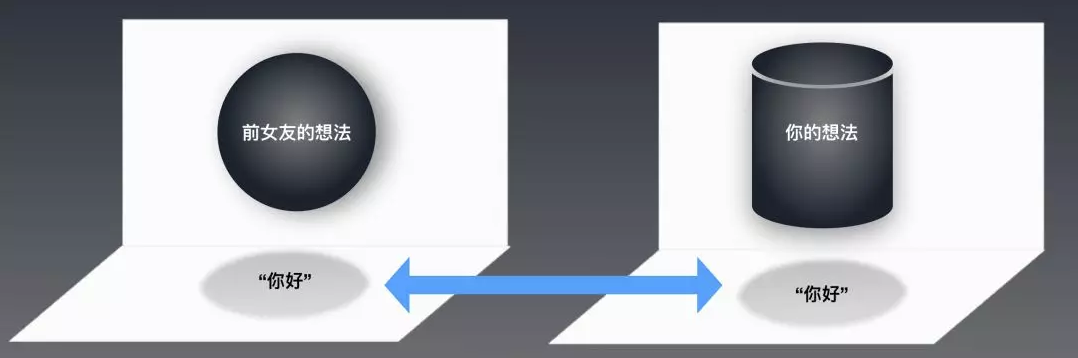
\includegraphics{img/mind.png}

\begin{quote}
你在想(圆柱):一年多不见了,她还好么?

前女友在想(球):这个人好眼熟,好像认识\ldots{}
\end{quote}

    以下指代词具体指代了什么?

\begin{quote}
A. ``四川火锅比日料更好,因为\textbf{它}很辣'';

B. ``四川火锅比日料更好,因为\textbf{它}不辣'';

C. 议员们拒绝给抗议者颁发许可证,因为\textbf{他们}害怕暴力

D. 议员们拒绝给抗议者颁发许可证,因为\textbf{他们}提倡暴力
\end{quote}

明文(含上下文)+ 场景模型(Context)+ 世界模型

    \hypertarget{ux600eux6837ux5b66ux4e60ux4ebaux5de5ux667aux80fd}{%
\section{怎样学习``人工智能''?}\label{ux600eux6837ux5b66ux4e60ux4ebaux5de5ux667aux80fd}}

最重要的能力:

\begin{itemize}
\item
  探索欲与耐心 ⋆⋆⋆⋆⋆
\item
  编程能力 ⋆⋆⋆
\item
  英语阅读能力 ⋆⋆⋆⋆
\item
  数学知识(线性代数、微积分、概率统计) +++
\end{itemize}

    有用的工具/教材:

\begin{itemize}
\item
  阅读别人的代码(Github/Kaggle) ⋆⋆⋆⋆
\item
  各类书籍与课程(数学之美/李宏毅深度学习/吴恩达机器学习) ⋆⋆⋆
\item
  一个好用的``梯子'' ⋆⋆⋆⋆⋆
\item
  colab ⋆⋆⋆⋆
\item
  四路泰坦 +++
\end{itemize}

    以吴恩达深度学习为例:

\begin{itemize}
\tightlist
\item
  \href{https://study.163.com/provider/2001053000/index.htm}{deeplearning.ai
  - 主页 - 网易云课堂}
\item
  \href{https://github.com/bighuang624/Andrew-Ng-Deep-Learning-notes}{github课程笔记}
\end{itemize}

视频 + 课程笔记 + 代码notebook

    通过参与竞赛进行学习:

\begin{itemize}
\tightlist
\item
  \href{https://www.kaggle.com/c/dogs-vs-cats-redux-kernels-edition}{猫狗大战}
\item
  \href{https://www.kaggle.com/jeffd23/catdognet-keras-convnet-starter}{查看别人的kernel}
\item
  \href{https://zhuanlan.zhihu.com/p/51889181}{知乎解析}
\end{itemize}

    \hypertarget{ux673aux5668ux5b66ux4e60ux662fux5982ux4f55ux5de5ux4f5cux7684}{%
\section{机器学习是如何工作的?}\label{ux673aux5668ux5b66ux4e60ux662fux5982ux4f55ux5de5ux4f5cux7684}}


\includegraphics{img/cake.png}

    如何分开红点与蓝点? 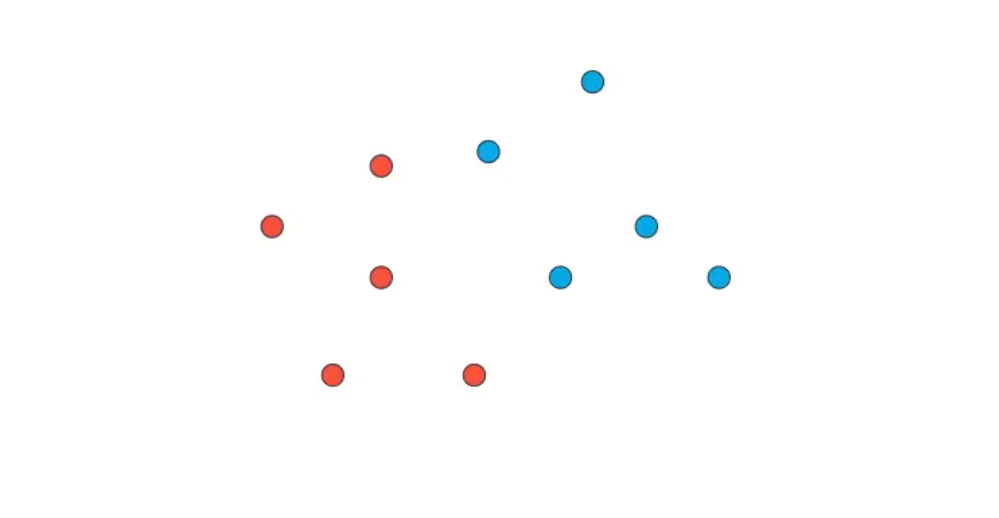
\includegraphics{img/scatter.png}

    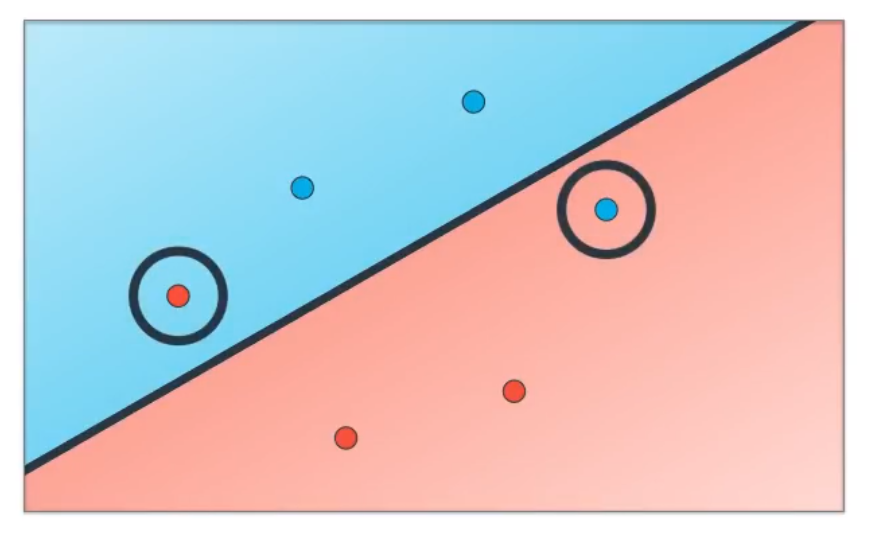
\includegraphics{img/2error.png}

    通常我们称之为 损失函数(loss) 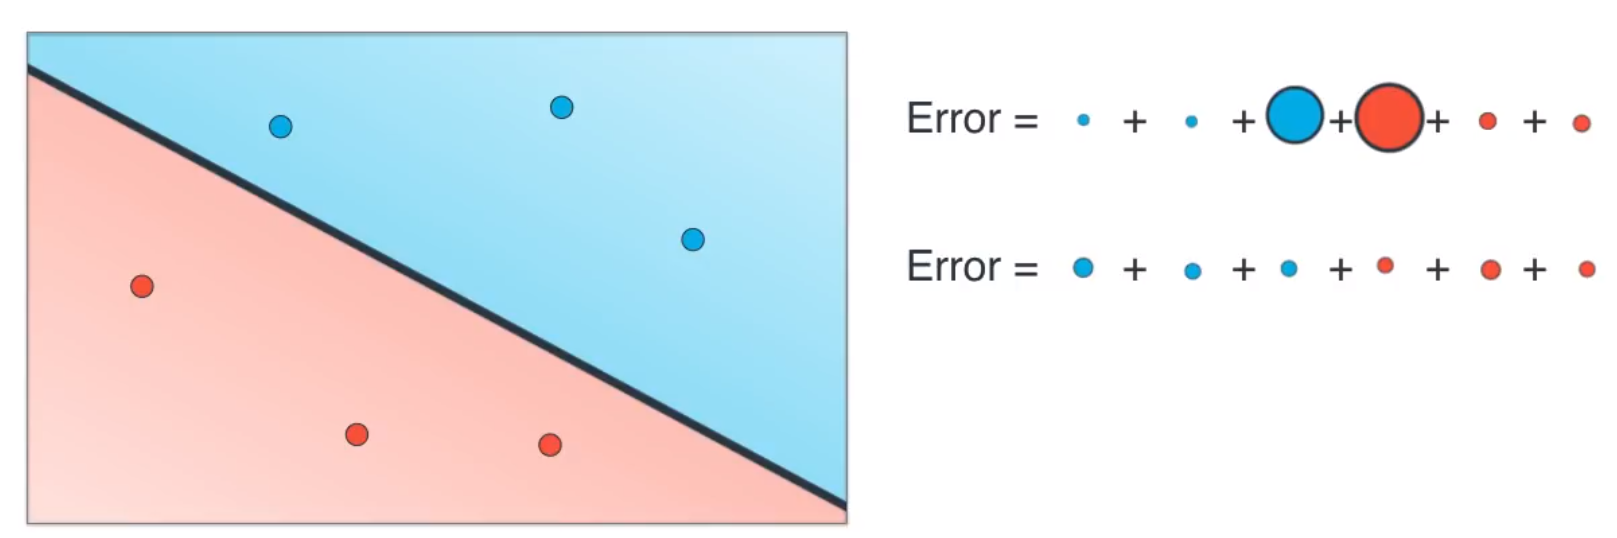
\includegraphics{img/error.png}

    随机梯度下降 \includegraphics{img/perceptron_animation.gif}
\includegraphics{img/fig5.gif}

    非线性问题 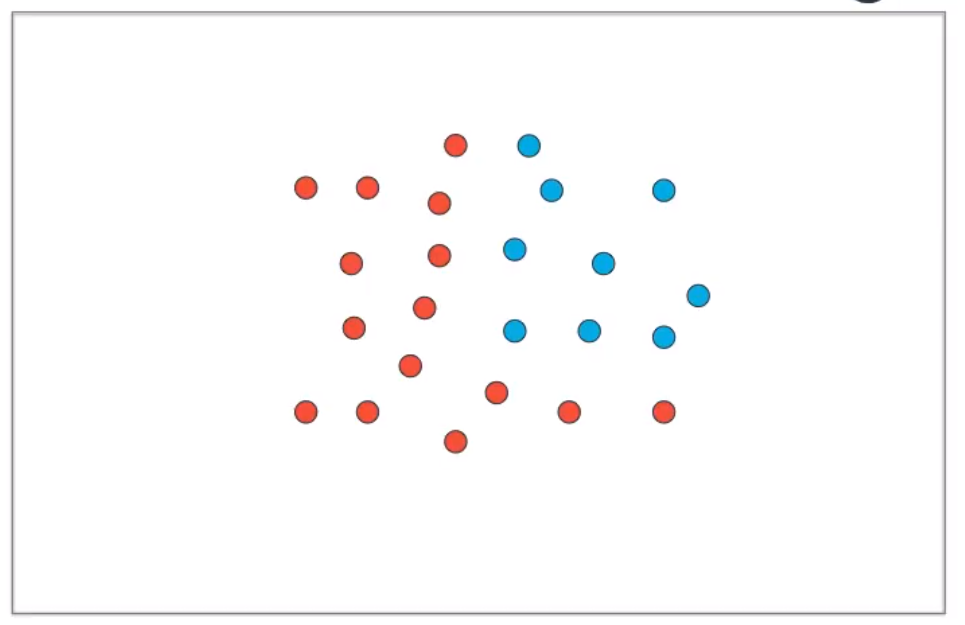
\includegraphics{img/nonlinear.png}

    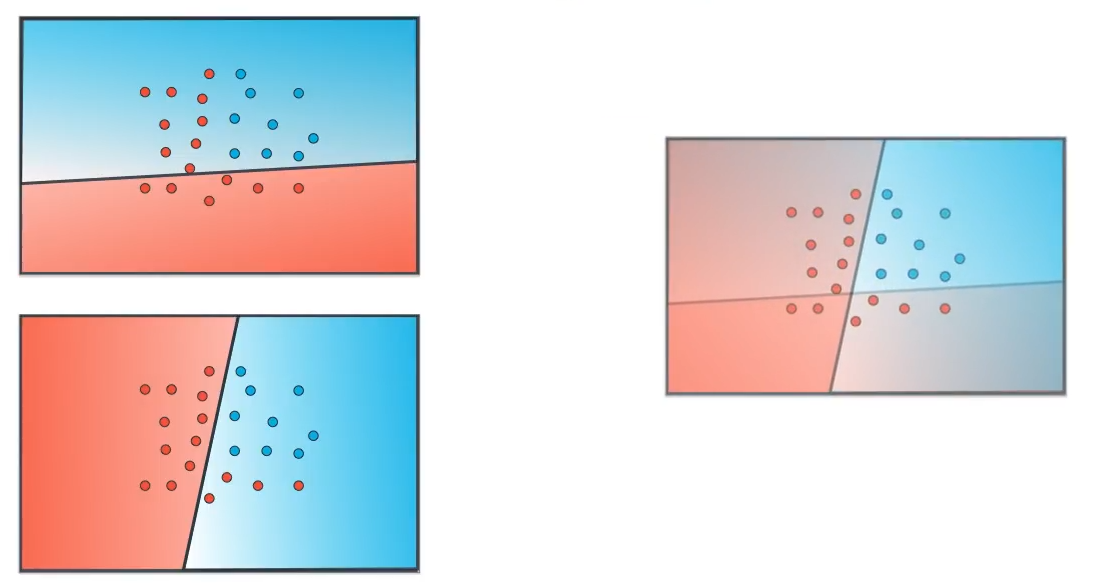
\includegraphics{img/combine.png}

    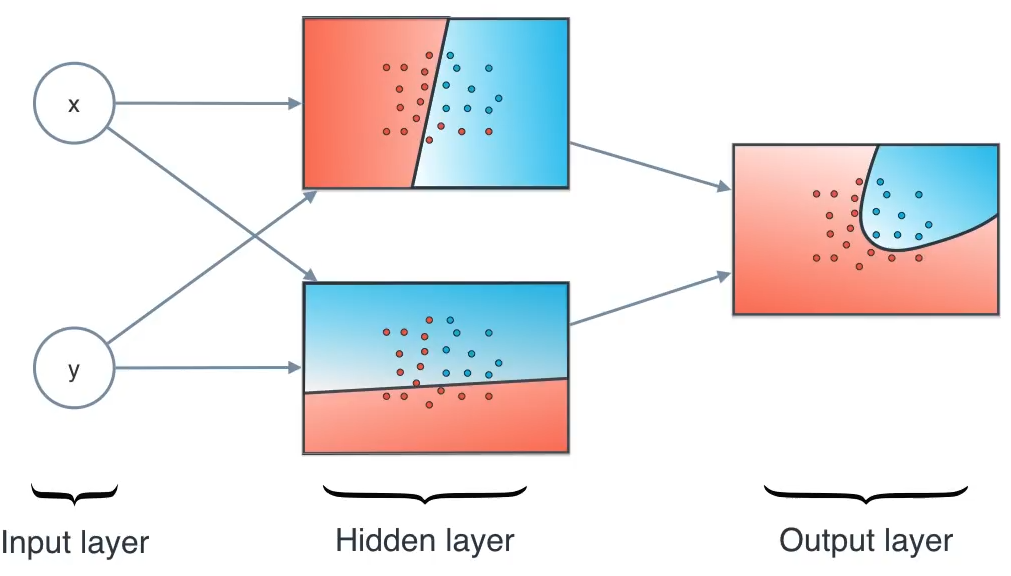
\includegraphics{img/model.png}

    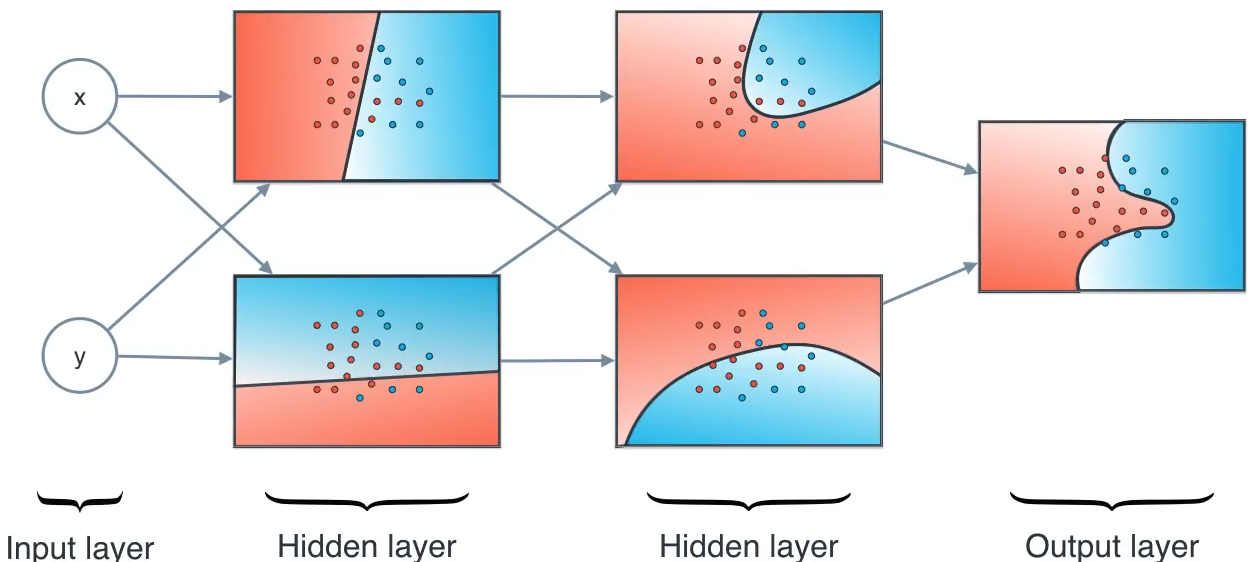
\includegraphics{img/deep.png}

    \hypertarget{hello-world-in-deep-learning}{%
\section{``Hello World'' in deep
learning}\label{hello-world-in-deep-learning}}

    \begin{Verbatim}[commandchars=\\\{\}]
{\color{incolor}In [{\color{incolor}2}]:} \PY{n}{plot\PYZus{}images\PYZus{}labels\PYZus{}predict}\PY{p}{(}\PY{n}{X\PYZus{}train\PYZus{}image}\PY{p}{,} \PY{n}{y\PYZus{}train\PYZus{}label}\PY{p}{,} \PY{p}{[}\PY{p}{]}\PY{p}{,} \PY{l+m+mi}{0}\PY{p}{,} \PY{l+m+mi}{20}\PY{p}{)}
\end{Verbatim}


    \begin{center}
    \adjustimage{max size={0.9\linewidth}{0.9\paperheight}}{output_39_0.png}
    \end{center}
    { \hspace*{\fill} \\}
    
    将原本 28x28 的图片转换为 1x728的向量 \includegraphics{img/reshape.gif}

    \hypertarget{ux7b2cux4e00ux6b65ux6784ux5efaux7f51ux7edcux5b9aux4e49ux4e00ux6279ux51fdux6570}{%
\subsection{第一步,构建网络(定义一批函数)}\label{ux7b2cux4e00ux6b65ux6784ux5efaux7f51ux7edcux5b9aux4e49ux4e00ux6279ux51fdux6570}}

    \begin{Verbatim}[commandchars=\\\{\}]
{\color{incolor}In [{\color{incolor}2}]:} \PY{k+kn}{import} \PY{n+nn}{numpy} \PY{k}{as} \PY{n+nn}{np}
        \PY{k+kn}{import} \PY{n+nn}{pandas} \PY{k}{as} \PY{n+nn}{pd}
        \PY{k+kn}{from} \PY{n+nn}{keras}\PY{n+nn}{.}\PY{n+nn}{utils} \PY{k}{import} \PY{n}{np\PYZus{}utils}  \PY{c+c1}{\PYZsh{} 用來後續將 label 標籤轉為 one\PYZhy{}hot\PYZhy{}encoding}
        
        \PY{n}{np}\PY{o}{.}\PY{n}{random}\PY{o}{.}\PY{n}{seed}\PY{p}{(}\PY{l+m+mi}{10}\PY{p}{)}
        \PY{k+kn}{from} \PY{n+nn}{keras}\PY{n+nn}{.}\PY{n+nn}{datasets} \PY{k}{import} \PY{n}{mnist}
        
        \PY{p}{(}\PY{n}{X\PYZus{}train\PYZus{}image}\PY{p}{,} \PY{n}{y\PYZus{}train\PYZus{}label}\PY{p}{)}\PY{p}{,} \PY{p}{(}\PY{n}{X\PYZus{}test\PYZus{}image}\PY{p}{,} \PY{n}{y\PYZus{}test\PYZus{}label}\PY{p}{)} \PY{o}{=} \PY{n}{mnist}\PY{o}{.}\PY{n}{load\PYZus{}data}\PY{p}{(}\PY{p}{)}
        
        \PY{k+kn}{import} \PY{n+nn}{matplotlib}\PY{n+nn}{.}\PY{n+nn}{pyplot} \PY{k}{as} \PY{n+nn}{plt}
        \PY{k}{def} \PY{n+nf}{plot\PYZus{}image}\PY{p}{(}\PY{n}{image}\PY{p}{)}\PY{p}{:}
            \PY{n}{fig} \PY{o}{=} \PY{n}{plt}\PY{o}{.}\PY{n}{gcf}\PY{p}{(}\PY{p}{)}
            \PY{n}{fig}\PY{o}{.}\PY{n}{set\PYZus{}size\PYZus{}inches}\PY{p}{(}\PY{l+m+mi}{2}\PY{p}{,} \PY{l+m+mi}{2}\PY{p}{)}
            \PY{n}{plt}\PY{o}{.}\PY{n}{imshow}\PY{p}{(}\PY{n}{image}\PY{p}{,} \PY{n}{cmap}\PY{o}{=}\PY{l+s+s1}{\PYZsq{}}\PY{l+s+s1}{binary}\PY{l+s+s1}{\PYZsq{}}\PY{p}{)} \PY{c+c1}{\PYZsh{} cmap=\PYZsq{}binary\PYZsq{} 參數設定以黑白灰階顯示}
            \PY{n}{plt}\PY{o}{.}\PY{n}{show}\PY{p}{(}\PY{p}{)}
            
        \PY{k}{def} \PY{n+nf}{plot\PYZus{}images\PYZus{}labels\PYZus{}predict}\PY{p}{(}\PY{n}{images}\PY{p}{,} \PY{n}{labels}\PY{p}{,} \PY{n}{prediction}\PY{p}{,} \PY{n}{idx}\PY{p}{,} \PY{n}{num}\PY{o}{=}\PY{l+m+mi}{10}\PY{p}{)}\PY{p}{:}  
            \PY{n}{fig} \PY{o}{=} \PY{n}{plt}\PY{o}{.}\PY{n}{gcf}\PY{p}{(}\PY{p}{)}  
            \PY{n}{fig}\PY{o}{.}\PY{n}{set\PYZus{}size\PYZus{}inches}\PY{p}{(}\PY{l+m+mi}{12}\PY{p}{,} \PY{l+m+mi}{14}\PY{p}{)}  
            \PY{k}{if} \PY{n}{num} \PY{o}{\PYZgt{}} \PY{l+m+mi}{25}\PY{p}{:} \PY{n}{num} \PY{o}{=} \PY{l+m+mi}{25}  
            \PY{k}{for} \PY{n}{i} \PY{o+ow}{in} \PY{n+nb}{range}\PY{p}{(}\PY{l+m+mi}{0}\PY{p}{,} \PY{n}{num}\PY{p}{)}\PY{p}{:}  
                \PY{n}{ax}\PY{o}{=}\PY{n}{plt}\PY{o}{.}\PY{n}{subplot}\PY{p}{(}\PY{l+m+mi}{5}\PY{p}{,}\PY{l+m+mi}{5}\PY{p}{,} \PY{l+m+mi}{1}\PY{o}{+}\PY{n}{i}\PY{p}{)}  
                \PY{n}{ax}\PY{o}{.}\PY{n}{imshow}\PY{p}{(}\PY{n}{images}\PY{p}{[}\PY{n}{idx}\PY{p}{]}\PY{p}{,} \PY{n}{cmap}\PY{o}{=}\PY{l+s+s1}{\PYZsq{}}\PY{l+s+s1}{binary}\PY{l+s+s1}{\PYZsq{}}\PY{p}{)}  
                \PY{n}{title} \PY{o}{=} \PY{l+s+s2}{\PYZdq{}}\PY{l+s+s2}{l=}\PY{l+s+s2}{\PYZdq{}} \PY{o}{+} \PY{n+nb}{str}\PY{p}{(}\PY{n}{labels}\PY{p}{[}\PY{n}{idx}\PY{p}{]}\PY{p}{)}  
                \PY{k}{if} \PY{n+nb}{len}\PY{p}{(}\PY{n}{prediction}\PY{p}{)} \PY{o}{\PYZgt{}} \PY{l+m+mi}{0}\PY{p}{:}  
                    \PY{n}{title} \PY{o}{=} \PY{l+s+s2}{\PYZdq{}}\PY{l+s+s2}{l=}\PY{l+s+si}{\PYZob{}\PYZcb{}}\PY{l+s+s2}{,p=}\PY{l+s+si}{\PYZob{}\PYZcb{}}\PY{l+s+s2}{\PYZdq{}}\PY{o}{.}\PY{n}{format}\PY{p}{(}\PY{n+nb}{str}\PY{p}{(}\PY{n}{labels}\PY{p}{[}\PY{n}{idx}\PY{p}{]}\PY{p}{)}\PY{p}{,} \PY{n+nb}{str}\PY{p}{(}\PY{n}{prediction}\PY{p}{[}\PY{n}{idx}\PY{p}{]}\PY{p}{)}\PY{p}{)}  
                \PY{k}{else}\PY{p}{:}  
                    \PY{n}{title} \PY{o}{=} \PY{l+s+s2}{\PYZdq{}}\PY{l+s+s2}{l=}\PY{l+s+si}{\PYZob{}\PYZcb{}}\PY{l+s+s2}{\PYZdq{}}\PY{o}{.}\PY{n}{format}\PY{p}{(}\PY{n+nb}{str}\PY{p}{(}\PY{n}{labels}\PY{p}{[}\PY{n}{idx}\PY{p}{]}\PY{p}{)}\PY{p}{)}  
                \PY{n}{ax}\PY{o}{.}\PY{n}{set\PYZus{}title}\PY{p}{(}\PY{n}{title}\PY{p}{,} \PY{n}{fontsize}\PY{o}{=}\PY{l+m+mi}{10}\PY{p}{)}  
                \PY{n}{ax}\PY{o}{.}\PY{n}{set\PYZus{}xticks}\PY{p}{(}\PY{p}{[}\PY{p}{]}\PY{p}{)}\PY{p}{;} \PY{n}{ax}\PY{o}{.}\PY{n}{set\PYZus{}yticks}\PY{p}{(}\PY{p}{[}\PY{p}{]}\PY{p}{)}  
                \PY{n}{idx}\PY{o}{+}\PY{o}{=}\PY{l+m+mi}{1}  
            \PY{n}{plt}\PY{o}{.}\PY{n}{show}\PY{p}{(}\PY{p}{)}
            
        \PY{n}{x\PYZus{}Train} \PY{o}{=} \PY{n}{X\PYZus{}train\PYZus{}image}\PY{o}{.}\PY{n}{reshape}\PY{p}{(}\PY{l+m+mi}{60000}\PY{p}{,} \PY{l+m+mi}{28}\PY{o}{*}\PY{l+m+mi}{28}\PY{p}{)}\PY{o}{.}\PY{n}{astype}\PY{p}{(}\PY{l+s+s1}{\PYZsq{}}\PY{l+s+s1}{float32}\PY{l+s+s1}{\PYZsq{}}\PY{p}{)}
        \PY{n}{x\PYZus{}Test} \PY{o}{=} \PY{n}{X\PYZus{}test\PYZus{}image}\PY{o}{.}\PY{n}{reshape}\PY{p}{(}\PY{l+m+mi}{10000}\PY{p}{,} \PY{l+m+mi}{28}\PY{o}{*}\PY{l+m+mi}{28}\PY{p}{)}\PY{o}{.}\PY{n}{astype}\PY{p}{(}\PY{l+s+s1}{\PYZsq{}}\PY{l+s+s1}{float32}\PY{l+s+s1}{\PYZsq{}}\PY{p}{)}
        \PY{n+nb}{print}\PY{p}{(}\PY{l+s+s2}{\PYZdq{}}\PY{l+s+se}{\PYZbs{}t}\PY{l+s+s2}{[Info] xTrain: }\PY{l+s+si}{\PYZpc{}s}\PY{l+s+s2}{\PYZdq{}} \PY{o}{\PYZpc{}} \PY{p}{(}\PY{n+nb}{str}\PY{p}{(}\PY{n}{x\PYZus{}Train}\PY{o}{.}\PY{n}{shape}\PY{p}{)}\PY{p}{)}\PY{p}{)}
        \PY{n+nb}{print}\PY{p}{(}\PY{l+s+s2}{\PYZdq{}}\PY{l+s+se}{\PYZbs{}t}\PY{l+s+s2}{[Info] xTest: }\PY{l+s+si}{\PYZpc{}s}\PY{l+s+s2}{\PYZdq{}} \PY{o}{\PYZpc{}} \PY{p}{(}\PY{n+nb}{str}\PY{p}{(}\PY{n}{x\PYZus{}Test}\PY{o}{.}\PY{n}{shape}\PY{p}{)}\PY{p}{)}\PY{p}{)}
          
        \PY{c+c1}{\PYZsh{} Normalization}
        \PY{n}{x\PYZus{}Train\PYZus{}norm} \PY{o}{=} \PY{n}{x\PYZus{}Train}\PY{o}{/}\PY{l+m+mi}{255}
        \PY{n}{x\PYZus{}Test\PYZus{}norm} \PY{o}{=} \PY{n}{x\PYZus{}Test}\PY{o}{/}\PY{l+m+mi}{255}
        
        \PY{n}{y\PYZus{}TrainOneHot} \PY{o}{=} \PY{n}{np\PYZus{}utils}\PY{o}{.}\PY{n}{to\PYZus{}categorical}\PY{p}{(}\PY{n}{y\PYZus{}train\PYZus{}label}\PY{p}{)} \PY{c+c1}{\PYZsh{} 將 training 的 label 進行 one\PYZhy{}hot encoding}
        \PY{n}{y\PYZus{}TestOneHot} \PY{o}{=} \PY{n}{np\PYZus{}utils}\PY{o}{.}\PY{n}{to\PYZus{}categorical}\PY{p}{(}\PY{n}{y\PYZus{}test\PYZus{}label}\PY{p}{)} \PY{c+c1}{\PYZsh{} 將測試的 labels 進行 one\PYZhy{}hot encoding}
        
        \PY{n}{y\PYZus{}train\PYZus{}label}\PY{p}{[}\PY{l+m+mi}{0}\PY{p}{]} \PY{c+c1}{\PYZsh{} 檢視 training labels 第一個 label 的值}
        \PY{n}{y\PYZus{}TrainOneHot}\PY{p}{[}\PY{p}{:}\PY{l+m+mi}{1}\PY{p}{]} \PY{c+c1}{\PYZsh{} 檢視第一個 label 在 one\PYZhy{}hot encoding 後的結果, 會在第六個位置上為 1, 其他位置上為 0}
        
        \PY{k+kn}{from} \PY{n+nn}{keras}\PY{n+nn}{.}\PY{n+nn}{models} \PY{k}{import} \PY{n}{Sequential}  
        \PY{k+kn}{from} \PY{n+nn}{keras}\PY{n+nn}{.}\PY{n+nn}{layers} \PY{k}{import} \PY{n}{Dense}
        
        \PY{k+kn}{import} \PY{n+nn}{matplotlib}\PY{n+nn}{.}\PY{n+nn}{pyplot} \PY{k}{as} \PY{n+nn}{plt}  
        \PY{k}{def} \PY{n+nf}{show\PYZus{}train\PYZus{}history}\PY{p}{(}\PY{n}{train\PYZus{}history}\PY{p}{,} \PY{n}{train}\PY{p}{,} \PY{n}{validation}\PY{p}{)}\PY{p}{:}  
            \PY{n}{plt}\PY{o}{.}\PY{n}{plot}\PY{p}{(}\PY{n}{train\PYZus{}history}\PY{o}{.}\PY{n}{history}\PY{p}{[}\PY{n}{train}\PY{p}{]}\PY{p}{)}  
            \PY{n}{plt}\PY{o}{.}\PY{n}{plot}\PY{p}{(}\PY{n}{train\PYZus{}history}\PY{o}{.}\PY{n}{history}\PY{p}{[}\PY{n}{validation}\PY{p}{]}\PY{p}{)}  
            \PY{n}{plt}\PY{o}{.}\PY{n}{title}\PY{p}{(}\PY{l+s+s1}{\PYZsq{}}\PY{l+s+s1}{Train History}\PY{l+s+s1}{\PYZsq{}}\PY{p}{)}  
            \PY{n}{plt}\PY{o}{.}\PY{n}{ylabel}\PY{p}{(}\PY{n}{train}\PY{p}{)}  
            \PY{n}{plt}\PY{o}{.}\PY{n}{xlabel}\PY{p}{(}\PY{l+s+s1}{\PYZsq{}}\PY{l+s+s1}{Epoch}\PY{l+s+s1}{\PYZsq{}}\PY{p}{)}  
            \PY{n}{plt}\PY{o}{.}\PY{n}{legend}\PY{p}{(}\PY{p}{[}\PY{l+s+s1}{\PYZsq{}}\PY{l+s+s1}{train}\PY{l+s+s1}{\PYZsq{}}\PY{p}{,} \PY{l+s+s1}{\PYZsq{}}\PY{l+s+s1}{validation}\PY{l+s+s1}{\PYZsq{}}\PY{p}{]}\PY{p}{,} \PY{n}{loc}\PY{o}{=}\PY{l+s+s1}{\PYZsq{}}\PY{l+s+s1}{upper left}\PY{l+s+s1}{\PYZsq{}}\PY{p}{)}  
            \PY{n}{plt}\PY{o}{.}\PY{n}{show}\PY{p}{(}\PY{p}{)}
\end{Verbatim}


    \begin{Verbatim}[commandchars=\\\{\}]
Using TensorFlow backend.

    \end{Verbatim}

    \begin{Verbatim}[commandchars=\\\{\}]
	[Info] xTrain: (60000, 784)
	[Info] xTest: (10000, 784)

    \end{Verbatim}

    \begin{Verbatim}[commandchars=\\\{\}]
{\color{incolor}In [{\color{incolor}7}]:} \PY{n}{model} \PY{o}{=} \PY{n}{Sequential}\PY{p}{(}\PY{p}{)}  \PY{c+c1}{\PYZsh{} 定义一个新模型}
        \PY{n}{model}\PY{o}{.}\PY{n}{add}\PY{p}{(}\PY{n}{Dense}\PY{p}{(}\PY{n}{units}\PY{o}{=}\PY{l+m+mi}{256}\PY{p}{,} \PY{n}{input\PYZus{}dim}\PY{o}{=}\PY{l+m+mi}{784}\PY{p}{,} \PY{n}{kernel\PYZus{}initializer}\PY{o}{=}\PY{l+s+s1}{\PYZsq{}}\PY{l+s+s1}{normal}\PY{l+s+s1}{\PYZsq{}}\PY{p}{,} \PY{n}{activation}\PY{o}{=}\PY{l+s+s1}{\PYZsq{}}\PY{l+s+s1}{relu}\PY{l+s+s1}{\PYZsq{}}\PY{p}{)}\PY{p}{)} \PY{c+c1}{\PYZsh{}定义一个256维的隐藏层}
        \PY{n}{model}\PY{o}{.}\PY{n}{add}\PY{p}{(}\PY{n}{Dense}\PY{p}{(}\PY{n}{units}\PY{o}{=}\PY{l+m+mi}{10}\PY{p}{,} \PY{n}{kernel\PYZus{}initializer}\PY{o}{=}\PY{l+s+s1}{\PYZsq{}}\PY{l+s+s1}{normal}\PY{l+s+s1}{\PYZsq{}}\PY{p}{,} \PY{n}{activation}\PY{o}{=}\PY{l+s+s1}{\PYZsq{}}\PY{l+s+s1}{softmax}\PY{l+s+s1}{\PYZsq{}}\PY{p}{)}\PY{p}{)} \PY{c+c1}{\PYZsh{} 定义一个10维的输出层}
\end{Verbatim}


    \includegraphics{https://3.bp.blogspot.com/-TpTfcbPRWWY/WVW-EUCKVLI/AAAAAAAAWuE/sn9sX6qMc38UePENvSmmgLH3bA7za-3ogCLcBGAs/s1600/3946_3.PNG}

    \hypertarget{ux7b2cux4e8cux6b65ux5b9aux4e49ux5b66ux4e60ux76eeux6807ux8861ux91cfux65b9ux6cd5}{%
\subsection{第二步,定义学习目标(衡量方法)}\label{ux7b2cux4e8cux6b65ux5b9aux4e49ux5b66ux4e60ux76eeux6807ux8861ux91cfux65b9ux6cd5}}

    \begin{Verbatim}[commandchars=\\\{\}]
{\color{incolor}In [{\color{incolor}8}]:} \PY{n}{model}\PY{o}{.}\PY{n}{compile}\PY{p}{(}\PY{n}{loss}\PY{o}{=}\PY{l+s+s1}{\PYZsq{}}\PY{l+s+s1}{categorical\PYZus{}crossentropy}\PY{l+s+s1}{\PYZsq{}}\PY{p}{,} \PY{n}{optimizer}\PY{o}{=}\PY{l+s+s1}{\PYZsq{}}\PY{l+s+s1}{SGD}\PY{l+s+s1}{\PYZsq{}}\PY{p}{,} \PY{n}{metrics}\PY{o}{=}\PY{p}{[}\PY{l+s+s1}{\PYZsq{}}\PY{l+s+s1}{accuracy}\PY{l+s+s1}{\PYZsq{}}\PY{p}{]}\PY{p}{)}
\end{Verbatim}


    参数说明: * \textbf{loss} : 使用 cross\_entropy (Cross entropy) 交叉熵.
\includegraphics{https://wikimedia.org/api/rest_v1/media/math/render/svg/0cb6da032ab424eefdca0884cd4113fe578f4293}
* \textbf{optimizer} : 随机梯度下降. * \textbf{metrics} :
使用准确率进行评估

    \hypertarget{ux7b2cux4e09ux6b65ux8badux7ec3ux7ec4ux5408ux6700ux5408ux9002ux7684ux65b9ux7a0b}{%
\subsection{第三步,训练!(组合最合适的方程)}\label{ux7b2cux4e09ux6b65ux8badux7ec3ux7ec4ux5408ux6700ux5408ux9002ux7684ux65b9ux7a0b}}

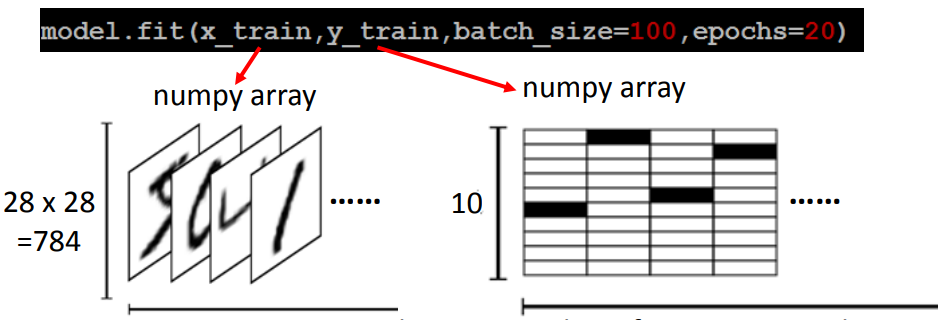
\includegraphics{img/fit.png}

    \begin{Verbatim}[commandchars=\\\{\}]
{\color{incolor}In [{\color{incolor}10}]:} \PY{n}{train\PYZus{}history} \PY{o}{=} \PY{n}{model}\PY{o}{.}\PY{n}{fit}\PY{p}{(}\PY{n}{x}\PY{o}{=}\PY{n}{x\PYZus{}Train\PYZus{}norm}\PY{p}{,} \PY{n}{y}\PY{o}{=}\PY{n}{y\PYZus{}TrainOneHot}\PY{p}{,} \PY{n}{validation\PYZus{}split}\PY{o}{=}\PY{l+m+mf}{0.2}\PY{p}{,} \PY{n}{epochs}\PY{o}{=}\PY{l+m+mi}{10}\PY{p}{,} \PY{n}{batch\PYZus{}size}\PY{o}{=}\PY{l+m+mi}{200}\PY{p}{,} \PY{n}{verbose}\PY{o}{=}\PY{l+m+mi}{2}\PY{p}{)}
\end{Verbatim}


    \begin{Verbatim}[commandchars=\\\{\}]
Train on 48000 samples, validate on 12000 samples
Epoch 1/10
 - 10s - loss: 1.7616 - acc: 0.5939 - val\_loss: 1.2360 - val\_acc: 0.7819
Epoch 2/10
 - 1s - loss: 0.9825 - acc: 0.7996 - val\_loss: 0.7536 - val\_acc: 0.8397
Epoch 3/10
 - 1s - loss: 0.6926 - acc: 0.8385 - val\_loss: 0.5820 - val\_acc: 0.8612
Epoch 4/10
 - 1s - loss: 0.5707 - acc: 0.8586 - val\_loss: 0.4971 - val\_acc: 0.8764
Epoch 5/10
 - 1s - loss: 0.5032 - acc: 0.8712 - val\_loss: 0.4470 - val\_acc: 0.8824
Epoch 6/10
 - 1s - loss: 0.4600 - acc: 0.8787 - val\_loss: 0.4140 - val\_acc: 0.8890
Epoch 7/10
 - 1s - loss: 0.4299 - acc: 0.8845 - val\_loss: 0.3898 - val\_acc: 0.8930
Epoch 8/10
 - 1s - loss: 0.4073 - acc: 0.8895 - val\_loss: 0.3720 - val\_acc: 0.8967
Epoch 9/10
 - 1s - loss: 0.3895 - acc: 0.8935 - val\_loss: 0.3575 - val\_acc: 0.9003
Epoch 10/10
 - 1s - loss: 0.3750 - acc: 0.8968 - val\_loss: 0.3462 - val\_acc: 0.9036

    \end{Verbatim}

    \begin{Verbatim}[commandchars=\\\{\}]
{\color{incolor}In [{\color{incolor}6}]:} \PY{n}{show\PYZus{}train\PYZus{}history}\PY{p}{(}\PY{n}{train\PYZus{}history}\PY{p}{,} \PY{l+s+s1}{\PYZsq{}}\PY{l+s+s1}{acc}\PY{l+s+s1}{\PYZsq{}}\PY{p}{,} \PY{l+s+s1}{\PYZsq{}}\PY{l+s+s1}{val\PYZus{}acc}\PY{l+s+s1}{\PYZsq{}}\PY{p}{)}
\end{Verbatim}


    \begin{center}
    \adjustimage{max size={0.9\linewidth}{0.9\paperheight}}{output_50_0.png}
    \end{center}
    { \hspace*{\fill} \\}
    
    \begin{Verbatim}[commandchars=\\\{\}]
{\color{incolor}In [{\color{incolor}7}]:} \PY{n}{show\PYZus{}train\PYZus{}history}\PY{p}{(}\PY{n}{train\PYZus{}history}\PY{p}{,} \PY{l+s+s1}{\PYZsq{}}\PY{l+s+s1}{loss}\PY{l+s+s1}{\PYZsq{}}\PY{p}{,} \PY{l+s+s1}{\PYZsq{}}\PY{l+s+s1}{val\PYZus{}loss}\PY{l+s+s1}{\PYZsq{}}\PY{p}{)}
\end{Verbatim}


    \begin{center}
    \adjustimage{max size={0.9\linewidth}{0.9\paperheight}}{output_51_0.png}
    \end{center}
    { \hspace*{\fill} \\}
    
    \hypertarget{ux5bf9ux7ed3ux679cux8fdbux884cux6d4bux8bd5}{%
\subsection{对结果进行测试}\label{ux5bf9ux7ed3ux679cux8fdbux884cux6d4bux8bd5}}

    \begin{Verbatim}[commandchars=\\\{\}]
{\color{incolor}In [{\color{incolor}8}]:} \PY{n}{scores} \PY{o}{=} \PY{n}{model}\PY{o}{.}\PY{n}{evaluate}\PY{p}{(}\PY{n}{x\PYZus{}Test\PYZus{}norm}\PY{p}{,} \PY{n}{y\PYZus{}TestOneHot}\PY{p}{)}  
        \PY{n+nb}{print}\PY{p}{(}\PY{l+s+s2}{\PYZdq{}}\PY{l+s+se}{\PYZbs{}t}\PY{l+s+s2}{[Info] Accuracy of testing data = }\PY{l+s+si}{\PYZob{}:2.1f\PYZcb{}}\PY{l+s+s2}{\PYZpc{}}\PY{l+s+s2}{\PYZdq{}}\PY{o}{.}\PY{n}{format}\PY{p}{(}\PY{n}{scores}\PY{p}{[}\PY{l+m+mi}{1}\PY{p}{]}\PY{o}{*}\PY{l+m+mf}{100.0}\PY{p}{)}\PY{p}{)}
\end{Verbatim}


    \begin{Verbatim}[commandchars=\\\{\}]
10000/10000 [==============================] - 0s 38us/step
	[Info] Accuracy of testing data = 90.5\%

    \end{Verbatim}

    \begin{Verbatim}[commandchars=\\\{\}]
{\color{incolor}In [{\color{incolor}9}]:} \PY{n}{prediction} \PY{o}{=} \PY{n}{model}\PY{o}{.}\PY{n}{predict\PYZus{}classes}\PY{p}{(}\PY{n}{x\PYZus{}Test\PYZus{}norm}\PY{p}{)}  \PY{c+c1}{\PYZsh{} Making prediction and save result to prediction  }
        \PY{n+nb}{print}\PY{p}{(}\PY{l+s+s2}{\PYZdq{}}\PY{l+s+si}{\PYZpc{}s}\PY{l+s+se}{\PYZbs{}n}\PY{l+s+s2}{\PYZdq{}} \PY{o}{\PYZpc{}} \PY{p}{(}\PY{n}{prediction}\PY{p}{[}\PY{l+m+mi}{240}\PY{p}{:}\PY{l+m+mi}{250}\PY{p}{]}\PY{p}{)}\PY{p}{)}  
          
        \PY{n}{plot\PYZus{}images\PYZus{}labels\PYZus{}predict}\PY{p}{(}\PY{n}{X\PYZus{}test\PYZus{}image}\PY{p}{,} \PY{n}{y\PYZus{}test\PYZus{}label}\PY{p}{,} \PY{n}{prediction}\PY{p}{,} \PY{n}{idx}\PY{o}{=}\PY{l+m+mi}{300}\PY{p}{)}
\end{Verbatim}


    \begin{Verbatim}[commandchars=\\\{\}]
[5 8 8 4 2 6 0 6 4 2]


    \end{Verbatim}

    \begin{center}
    \adjustimage{max size={0.9\linewidth}{0.9\paperheight}}{output_54_1.png}
    \end{center}
    { \hspace*{\fill} \\}
    

    % Add a bibliography block to the postdoc
    
    
    
    \end{document}
